\documentclass[aspectratio=1610]{beamer}
\beamertemplatenavigationsymbolsempty
\setbeamertemplate{footline}[frame number]
\graphicspath{ {./images/} }
\usetheme{Rochester}

\usepackage{graphicx} % Required for inserting images

\title{1D SDC - a Layered DAG}
\author{Jerry Kiely}
\date{October 2026}

\begin{document}

\begin{frame}
\titlepage
\end{frame}




\begin{frame}
\frametitle{Questions}
While implementing Ahmed's \textit{minimum free energy} algorithm in
Python, I started to consider the possibility that the calculated value
may have come from a configuration different to the
\textit{target configuration}.
\newline

I wanted a way to see what actual configuration resulted in the
\textit{minimum free energy} at a specific temperature, to confirm
that the calculated value came from the \textit{target configuration}.
\newline

Is the \textit{target configuration} always the most
\textit{thermodynamically favoured configuration} for all
temperatures?
\end{frame}




\begin{frame}
\frametitle{MFE}
The \textit{dynamic programming} approach to calculating the
\textit{minimum free energy} of a 1D SDC
\newline

\begin{itemize}
    \item $N$ positions
    \item $\leq k$ tiles per position
    \item $\mathcal{O}(Nk^2)$
\end{itemize}
\hfill \break

The algorithm calculates the \textit{minimum free energy}, but does not
provide the configuration that resulted in the \textit{minimum free energy}.
Therefore the calculation is a black box.
\newline

How do we know what configuration resulted in the calculated value of
the \textit{minimum free energy}, and if this configuration is indeed
the \textit{target configuration}?
\end{frame}




\begin{frame}
\frametitle{DAG}
A Directed Acyclic Graph
\newline

\begin{columns}
    \column{0.45\textwidth}
        \begin{itemize}
            \item Nodes
            \item Directed Edges
            \item No Cycles
        \end{itemize}
    \column{0.55\textwidth}
        \begin{figure}
            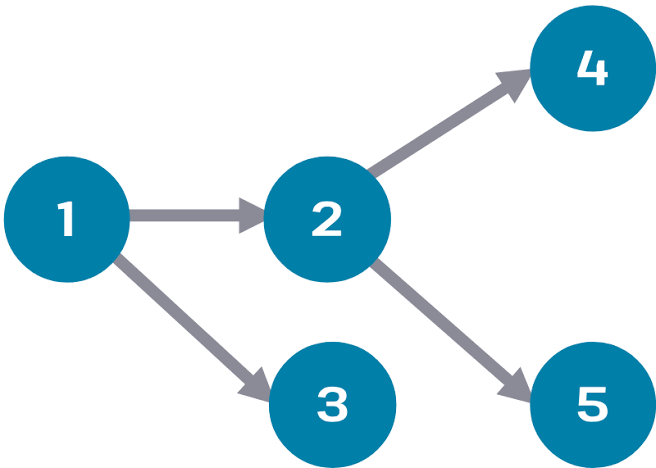
\includegraphics[scale=0.25]{DAG}
        \end{figure}
\end{columns}

\end{frame}




\begin{frame}
\frametitle{Layered DAG}
A Layered DAG
\newline

\begin{columns}
    \column{0.45\textwidth}
        \begin{itemize}
            \item Directed Acyclic Graph
            \item Partitioned into Layers
            \item Topological Ordering
        \end{itemize}
    \column{0.55\textwidth}
        \begin{figure}
            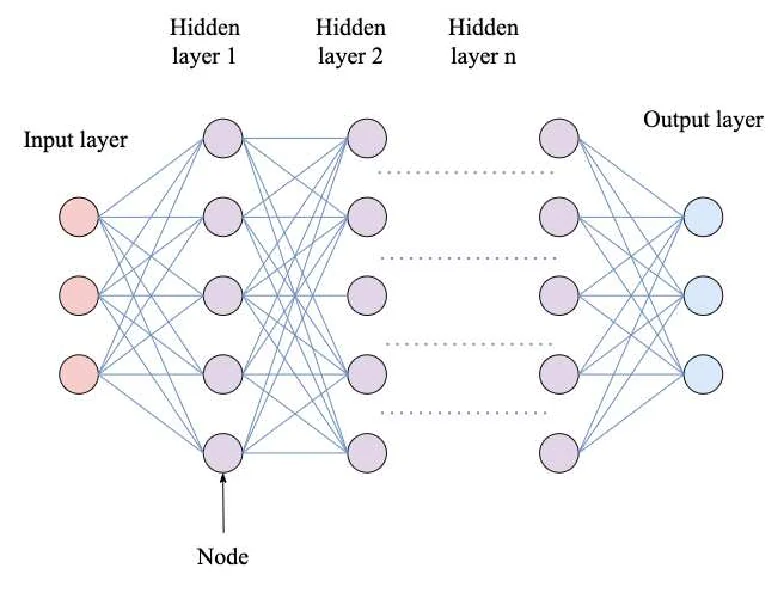
\includegraphics[scale=0.25]{Layered DAG}
        \end{figure}
\end{columns}

\end{frame}




\begin{frame}
\frametitle{Features of a Layered DAG}
Why is a Layered DAG relevant to 1D SDC?
\newline

\begin{columns}
    \column{0.75\textwidth}
        \begin{itemize}
            \item Competing tiles occupy Layers ($L_i$)
            \item Layers are ordered ($L_i < L_j$ when $i < j$)
            \item A tile from $L_i$ binds with a tile from $L_{i + 1}$
            \item Edges connect tiles from layer $i$ to layer $i + 1$
            \item Edges connect tiles with weight $\Delta G (T, r^m_i, l^n_{i + 1})$
        \end{itemize}
    \column{0.25\textwidth}
        \begin{figure}
            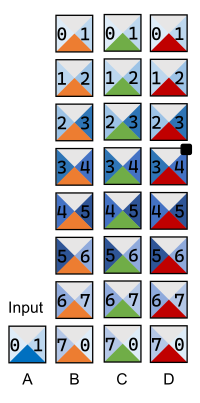
\includegraphics[scale=0.35]{1D SDC}
        \end{figure}
\end{columns}

\end{frame}




\begin{frame}
\frametitle{MFE and Thermodynamic Favourability}
For a Tileset represented as a Layered DAG, the Shortest Path gives
you the most \textit{thermodynamically favoured configuration} at a
specific temperature.
\newline

If this configuration is the \textit{target configuration}, then the
Shortest Path is the \textit{free energy} of the
\textit{target configuration}, and the \textit{minimum free energy}
of the Tileset.
\end{frame}




\begin{frame}
\frametitle{Layered DAG Traversal}
The Shortest Path through a Layered DAG
\newline

\begin{columns}
    \column{0.35\textwidth}
        \begin{itemize}
            \item Topological Sort
            \item Edge Relaxation
        \end{itemize}
    \column{0.65\textwidth}
        \begin{figure}
            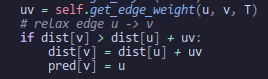
\includegraphics[scale=0.65]{Edge Relaxation}
        \end{figure}
\end{columns}
\hfill \break

Note: for a Layered DAG, the layers induce a \textit{topological ordering}, so
sorting is unnecessary.
\end{frame}




\begin{frame}
\frametitle{Comparison}
Comparison of approaches:
\newline

\begin{center}
    \setlength{\tabcolsep}{10pt}
    \renewcommand{\arraystretch}{1.5}
    \begin{tabular}{ |c|c|c| }
        \hline
        & Time Complexity & Space Complexity \\
        \hline
        DP & $\mathcal{O}(Nk^2)$ & $\mathcal{O}(k)$ \\
        \hline
        DAG & $\mathcal{O}(V + E)$ & $\mathcal{O}(V + E)$ \\
        \hline
        Layered DAG & $\mathcal{O}(E)$ & $\mathcal{O}(V + E)$ \\
        \hline
    \end{tabular}
\end{center}
\hfill \break

Note: For the Layered DAG, with respect to space complexity, we need
$E$ (the number of edges) space to hold the edges, and $V$ (the number
of vertices) space to hold the reconstructed path itself.
\end{frame}




\begin{frame}
\frametitle{A Note on Edges}
There are $k_{i}$ competing tiles in $L_{i}$
\newline

\begin{itemize}
    \item $k = \max_{i}(k_{i})$ tiles per position
    \item $\therefore $ at most $k^2$ possible bindings between tiles in consecutive positions
    \item $N$ positions
    % \item $N - 1$ binding between positions
    \item $(N - 1)k^2$ possible bindings between tiles across all positions
    \item $\therefore \text{ no more than } (N - 1)k^2$ edges
    \item $\therefore \mathcal{O}(E) = \mathcal{O}(Nk^2)$
\end{itemize}

\end{frame}




\begin{frame}
\frametitle{MFE - Code}

\begin{figure}
    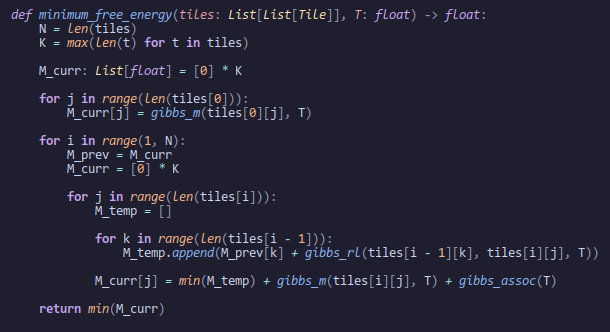
\includegraphics[scale=0.65]{MFE Code}
\end{figure}

\end{frame}




\begin{frame}
\frametitle{MFE - Test}

\begin{figure}
    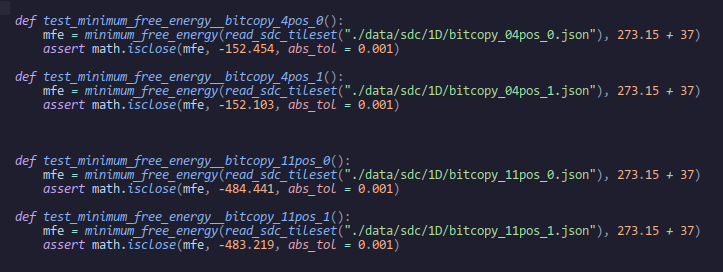
\includegraphics[scale=0.5]{MFE}
\end{figure}

\end{frame}




\begin{frame}
\frametitle{Shortest Path - Code}

\begin{figure}
    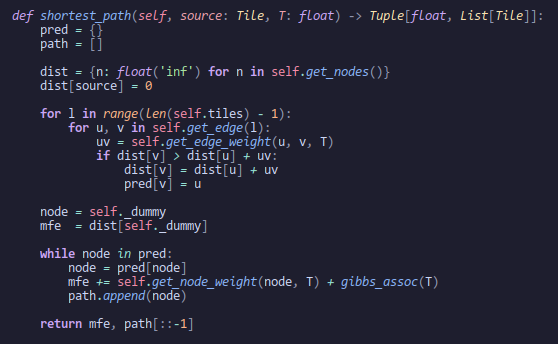
\includegraphics[scale=0.65]{Shortest Path Code}
\end{figure}

\end{frame}




\begin{frame}
\frametitle{Shortest Path - Test}

\begin{figure}
    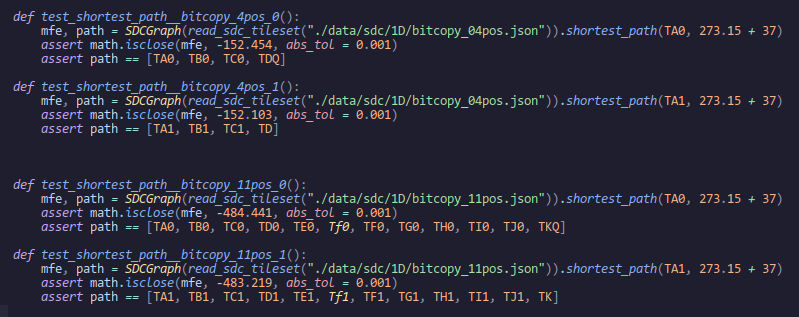
\includegraphics[scale=0.5]{Shortest Path}
\end{figure}

\end{frame}




\begin{frame}
\frametitle{Finally}
Next steps?
\newline

\begin{itemize}
    \item Multilayer Perceptron (MLP)
    \item Free Palestine!
\end{itemize}

\end{frame}




\begin{frame}
\frametitle{Goodbye}
Questions?
\end{frame}

\end{document}
